%%%%%%%%%%%%%%%%%%%%%%%%%%%%%%%%%%%%%
%%%%%%%%%%%%%%%%%%%%%%%%%%%%%%%%%%%%%
%%
%% Typeset by                  , Research Press, NRC
%% Date: 
%% NRC, <name of journal>
%% 
%%%%%%%%%%%%%%
%%
%% 1. See original preamble material (at bottom of file) for
%%    details on source of current .tex file: conversion
%%    from word-processing program or author-generated TeX
%%    code. 
%%
%% 2. This template includes most options and packages used by 
%%    all the NRC journals. UNcomment those packages and options
%%    which are REQUIRED. 
%% 
%%%%%%%%%%%%%%%%%%%%%%%%%%%%%%%%%%%%%
%%%%%%%%%%%%%%%%%%%%%%%%%%%%%%%%%%%%%


%% 1. Class file (nrc1 or nrc2) + options (see userguide, pp.1-2; p.9):
\documentclass[%% french,        %% use with \usepackage[french]{babel}
               %% leqno,         %% only for nrc1 (default is right eqno)
               %% reqno,         %% only for nrc2 (default is left eqno)
nonumbib,      %% biblio entries without nos.
%
               %% breakaddress,  %% linebreak btwn author(s) + address(es)
               %% twocolid,      %% IDbox spans 2 cols
               %% twocolid*,     %% 2-col IDbox
               %% preprint,      %% removes identifying nos. from headers/footers
               %% proof          %% `Proof/Epreuve' in footer
               %% pagnf,         %% `Pagination not final/Pagination non finale'
               %% trimmarks,     %% add trimmarks
               %% finalverso,    %% final blank verso NOT included in pagerange
]{nrc1}                          %% choose one: nrc1 or nrc2

%% NOTE: authors may use the following options, which should be
%%       DELETED once the file comes in-house:
%%      
%%       usecmfonts    type1rest     genTeX

\usepackage{lineno}


\usepackage{color}
\newcommand{\red}{\textcolor{red}}

%% 2. Frequently used packages -- see pp.2-3 of userguide: 
%%    a. graphics-related:
\usepackage{graphicx}       %% color not usually needed
\usepackage[figuresright]{rotating} %% for landscape tables

%%    b. math-related: 
\usepackage{amsmath}        %% math macros in wide use
%%    \usepackage{amssymb}        %% additional math symbols
%%    \usepackage{dcolumn}        %% decimal alignment for tables
%%    \usepackage{bm}             %% `bold math' via \bm command

%%    c. for website addresses:
%%    \usepackage{url}            %% inserts linebreaks automatically
%%    \NRCurl{url}

%%    d. biblio-related:
%\usepackage{cite}           %% enhances options for \cite commands
\usepackage[authoryear, round]{natbib}

%%    e. for English-language papers:
\usepackage[french,english]{babel}  

%%    f. for French-language papers: 
%%    \usepackage[english,french]{babel}  %% remember to add french as a
                                          %% CLASS option, above
%%    g. for ragged-right tables:
%%    \usepackage{array}
%%    \newcommand{\PreserveBackslash}[1]{\let\temp=\\#1\let\\=\temp}
%%    \let\PBS=\PreserveBackslash

%%    h. for left curly brace to span several lines of equations:
%%    \usepackage{cases}
%%    \expandafter\let\csname numc@left\expandafter\endcsname\csname 
%%                 z@\endcsname


%% 3. Resetting float parameters: 
%%    a. in nrc1:
%%    \renewcommand{\topfraction}{.95}
%%    \renewcommand{\textfraction}{.05}
%%    \renewcommand{\floatpagefraction}{.95}

%%    b. in nrc2:
%%    \renewcommand{\topfraction}{.95}
%%    \renewcommand{\floatpagefraction}{.95}
%%    \renewcommand{\dbltopfraction}{.95}
%%    \renewcommand{\textfraction}{.05}
%%    \renewcommand{\dblfloatpagefraction}{.95}


%% 4. Resetting journal-specific parameters:
%%    a. eqn nos. with section nos.:
%%    \numberby {equation}{section}
%%    \setcounter{equation}{0}

%%    b. in-line citations to use ( ) instead of default [ ]:
%%   \renewcommand{\citeleft}{(}
%%   \renewcommand{\citeright}{)}

%%    c. for JEES (to expand inter-line spacing; see p.12 of guide):
%%    \easebaselines


%% 5. Miscellaneous macros to always have available:
%%    a. shorthands:
\let\p=\phantom
\let\mc=\multicolumn

%%    b. struts for vertical spacing above/below rules in tables:
%%%%%%%%%%%%%%%%%%  beginning of Claudio Beccari's code:
%% Spacing commands for {tabular} (from TTN 2,3:10 -- Claudio
%%                                                    Beccari): 
%% Usage: a. use \T to put space below a line 
%%           (e.g., at top of a `cell' of text)
%%        b. use \B to put space above a line 
%%           (e.g., at bottom of a `cell' of text)
\newcommand\T{\rule{0pt}{2.6ex}}            % = `top' strut
\newcommand\B{\rule[-1.2ex]{0pt}{0pt}}      % = `bottom' strut
%%%%%%%%%%%%%%%%%%  end of Claudio's code 

%%%%%%%%%%%%%%%%%%%%%%%%%%%%%%%%%%%%%   end of class and package 
%%%%%%%%%%%%%%%%%%%%%%%%%%%%%%%%%%%%%   options, additional macros


%% Journal-specific information for opening page -- pp.9-11 of guide:
%% a. numbers:
\setcounter{page}{1}             %% replace 1 with starting page no.
\volyear{XX}{2001}               %% volume, year of journal 
\journal{}                       %% jrnl. abbrev. (see App.A of guide)
\journalcode{}                   %% jrnl. acro    (see App.A of guide)
\filenumber{}                    %% NRC file number
%% \filenumber*{}                %% prefixes \filenumber to all page nos.
                                 %% NOTE: COMMENT OUT class options
                                 %%             pagnf
                                 %%             proof
                                 %%       once no longer needed


%% b. dates:
\received{}                      %% insert date, no period
\revreceived{}                   %% <same>
\accepted{}                      %% <same>
\revaccepted{}                   %% <same>
%% \IDdates{}                       %% <same>. Use for `Revised ...' etc.
%% \webpub{}                        %% insert date
%% \commdate{}                      %% <same>


%% c. miscellaneous:
%%   \assoced{}                  %% insert name of Associate ed.
%%   \corred{}                   %% insert name of Corresponding ed.
%%   \dedication{}               %% insert text as neede
%%   \abbreviations{}            %% insert as needed

\linespread{2}

\begin{document}

%% Reversed titlebar -- see p.11 of userguide:
%% \specialtitle{}      %% for black stripe + text + regular title
%% \specialtitle*{}     %% black stripe + text only




%% Title, Author(s), Address(es) -- see p.4 of userguide for 
%%    various options to save time and keyboarding, esp. where
%%    authors share same address(s). 

\title{5th: Reframing Stock Assessment As Risk Management; An Management Strategy Evaluation for Atlantic Tuna
Risk is an uncertainty that matters.}

%% Author 1:
\author{Laurence T. Kell}        
\address{Centre for Environmental Policy, Imperial College London, London SW7 1N.}

\author{Rishi Sharma}        
\address{}

\author{Iago Mosqueira}        
\address{}

\author{Toshi Kitakado}        
\address{}

\shortauthor{Kell, et al.} %% for headers

%%%%%%%%
%% This line goes here in nrc1.
%% \maketitle			
%%%%%%%%


%% Abstract/Resume area -- see pp.5,12 of userguide:
%\begin{abstract}

%The Precautionary Approach (PA) requires that undesirable outcomes be anticipated and measures taken to reduce the probability of them occurring. This requires determining how well management measures achieve their objectives given uncertainty, i.e. to manage risk. %, i.e. with respect to the ability to assess and manage stocks, given their intrinsic variability and the occurrence of environmental events inherent to the system. 
%We therefore define stock assessment, consistent with the PA, as the description of the characteristics of a 'stock' so that its biological reaction to being exploited can be rationally predicted and the predictions tested. This requires a move away from stock assessment to the management of risk. We provide an example of how to do this using Management Strategy Evaluation, i.e. by determining under what conditions a simple stock assessment method, based on biomass, can be used to achieve management objectives. Although such models have been criticised as being too simplistic to capture the actual population dynamics we show that they can meet our definition of stock assessment. %by providing advice on stock status relative to reference points and predict the response of a stock to management. 
%A consequence of the adoption of the PA is that many more stocks have to be assessed. %Which in turn has resulted in the use of integrated models that can utilise more sources of data and information and an increased number of stock assessments for data poor and knowledge limited stocks. Which resulted in many stock assessment models require priors for population parameters such as r (the population growth rate at low population size). In the case of biomass base models these are commonly derived from age  based models. 
%We also show that 
%the population parameters derived from biomass and age based models are not equivalent and that 
%it is more important to develop priors for reference points used to provide management advice than for population parameters, such as population growth rate, used in the stock assessment model. 

%\end{abstract}

%\begin{resume}\end{resume}

\maketitle

\linenumbers
\linespread{2}

\newpage

\section*{Points}


We ran three MPs, i.e.

\begin{enumerate}
\item Biomass dynamic model based MP with q hockey stick HCR
\item Empirical HCR for trend in CPUE
\item Empirical HCR for relative difference in CPUE
\end{enumerate}
    

The Empirical HCRs performed best!, particularly the one using the trend.

The main points are

\begin{enumerate}
\item The MP used an OEM that modelled the actual fleets as fitted using MFCL, this is different from what was done by the ICCAT WG. This is an important point that needs emphasising since it impacts on what we can conclude and the implications for SCRS and the Commission.
\item The Empirical HCRs using CPUE, do better than the model based one
\item The two Empirical HCRs are based on the trend (D) and value relative to a reference level (P), i.e. P\&D of a PID controller. \item The next step will be to look at PID controllers within a generic framework
\item MSE can also be used to evaluate the value-of-information, i.e. if we resolved some uncertainty as represented by the OM, i.e. knew M or steepness would we reduce risk?
\item Can we ever resolve M and/or steepness hypotheses, do we need to if we use model-free MPs?
\item What is more important, the choice of OM or the random time series used in the simulations, I have some ideas on how to do this.
\end{enumerate}


% Iife history arguments have been used to show that the Schaefer production model is probably not appropriate for tunas (e.g. Fisheries Research 61 (1), 145-149), and something like a Pella-Tomlinson with BMSY<0.5B0 is probably more realistic (primarily due to high steepness).   admitting this asymmetry in the yield curve would admit that considerably lower levels of current depletion are possible.
%MSE can help add stability to the TAC decision process that industry can rely on rather than the whims of shifting political pressures. The stakeholder consultation is an essential part of the  MSE process. The MSE process can be used to guide the scientific process e.g. reducing many scientific uncertainties will make very little difference to the performance of a sensible feedback-based harvest control rule, but the simulation testing can help ensure that expenditure is prioritised to provide the best research (or monitoring/enforcement) value.

\section*{Introduction}

Management Strategy Evaluation (MSE) should consider 5 key elements of uncertainty, i) estimation error, ii) implementation error, iii) observation error, iv) process error and 5) model error. Currently, the tRFMO's are mainly focused on estimation, observation and process error. Implementation and model error is lacking from most tRFMO's other than CCSBT (Sharma et al. ???).  A reason for this is because to date the tRFMOs have mainly used a stock assessment paradigm as the basis for OM design, although this is a good starting point further processes, observation error and ecological processes with time dependence should be accounted for in OM designs to ensure robustness (tRFMO MSE WG). 


Management Strategy Evaluation (MSE) is increasingly being used to develop management procedures (MPs) and Harvest Control Rules (HCRs) to manage domestic fisheries, e.g. in South Africa and Australia. The tuna Regional Fisheries Management Ogranisations (tRFMOs) are now testing and in some limited cases have implemented MPs \citep{hillary2013sbthcr}. A reason for this is because MSE allows a fuller consideration of uncertainty as required by the Precautionary Approach \citep{garcia1996precautionary} and helps to provide stability since management objectives and management actions meet them have to be preagreed. MSE can also be used to guide the scientific process by identifying where the reduction of scientific uncertainties will improve management and so help to ensure that expenditure is priortised to provide the best research, monitoring, control  and surveillance \cite{fromentin2014spectre}. 

In MSE management strategies are simulation tested using an Operating Model (OM) which represents the resource dynamics and the uncertainty about them. The OM is projected forward using the MP as a feedback controller, where information about the difference between the system state and the desired reference level is used to alter the gap between them \citep{ramaprasad1983definition}. An MP is the combination of pre-defined data, together with an algorithm to which they are input to provide a value for an appropriate management control measure. Linking the OM and the MP requires an Observation Error Model (OEM) to generate fishery-dependent or fishery-independent resource monitoring data. The OEM reflects the uncertainties, between the actual dynamics of the resource and perceptions arising from observations and assumptions by modelling the differences between the measured value of a resource index and the actual value in the OM.  The intention is to demonstrate, through simulation trials, robust performance of the MP in the presence of uncertainties. 

There will always be a variety of aims when conducting an MSE, differences in knowledge and data, and challenges of how to deal with aleatoric and epistemic uncertainties, alternative ways to condition OMs and complexities of implementation. Conducting an MSE ideally requires a dialogue between managers, fishers, consumrs, environmentalists and scientists and involves a number of steps \citep{punt2007developing} namely:

\begin{enumerate}
 \item Identification of management objectives and mapping these to performance measures in order to quantify how well they have been achieved;
 \item Agreeing the main uncertainties about the resource dynamics and the selection of hypotheses for the OMs;
 \item Conditioning the OMs using data and knowledge and possible rejection and weighting of hypotheses;
 \item Identifying candidate management strategies and coding these in the form of an MP;
 \item Projecting the OMs forward using the OEM to generate psuedo data and the MPs as a feedback controller; and
 \item Agreeing the MP that best meets management objectives.
\end{enumerate}

Strictly speaking MSE is used to evaluate an MP that will be implemented exactly as simulation tested, i.e. the Revised Management Procedure (RMP) of the International Whaling Commission (IWC) or the MP adopted by the Commission for the Conservation of Southern Bluefin Tuna (CCSBT). The MP selected for implementation is the one that best meets the agreed management objectives, the MP does not have to make any pretence of actually modelling the resource dynamics. This is a common approach taken in engineering when developing feedback controllers which starts from measurements of the behavior of the system in response to external influences (inputs to the system) and then tries to determine a mathematical relation between them without going into the details of what is actually happening inside the system. An example is the empirical HCR of CCSBT, where trends in an index of catch per unit effort (CPUE) and an aerial survey are used to set catches. Even when using a model based MP, there does not have to be complete knowledge about the structure of system processes \cite{sohlberg2012supervision} as in the case of the IWCs RMP which at its core has a simple Pella-Tomlinson population model that nobody believed was remotely good as a population model but through simulation testing was shown to be able to robustly meet management objectives.

Simulation can also be used to evaluate the particular elements of an Management Procedure, for example to determine the knowledge and data requirements for a stock assessment, reference points  to provide robust advice  \citep[e.g.][]{kell2005flat,kell2005round}. Where a robust management system is one that still functions correctly in the presence of uncertainty or stressful environmental conditions \citep{radatz1990ieee}. In which case, however, even though elements of a procedure after testing are implemented this is not a MP.

One of the main reasons for the tRFMOs to conduct MSE is to develop HCRs in order to achieve Marine Stewardship Council (MSC) certification. Certification brings many benefits whcih include, ensuring that fisheries are sustainable, protecting livelihoods, help with marketing and securing a price premium. To achieve the MSC standard requires a large amount of technical knowledge and fishery information, and failure to meet the minimum requirements or to provide the necessary information may result in ‘conditions’ being placed on a fishery, which can increase the overall cost of achieving and maintaining certification. 

In general highly migratory pelagic stocks received more conditions than other fisheries \citep{bellchambers2016identifying}. For example the North Atlantic artisanal albacore fishery when it was certified in 2014 received a number of conditions related to HCRs. These included that by 2018 evidence must be presented that the stock is at or fluctuating around its target reference point and a well-defined HCR should be in place. The fishers were also required to work actively to achieve short and long-term objectives based on the sustainability of the resource. These were the main reasons for the International Commission for the Conservation of Atlantic Tunas (the inter-governmental fishery organisation responsible for the conservation of tunas and tuna-like species in the Atlantic Ocean and its adjacent seas) to conduct MSE for North Atlantic Albacore.


\newpage
\section{Material and Methods}

\subsection*{Case Study}

When North Atlantic albacore was assessed in 2013 two methods were used, Multifan-CL an integrated methods \citep{fournier1998mfcl} that can use the raw catch, effort and length compostion data  and a biomass dynamic stock models \cite[e.g.][]{prager1994suite} that used time series of catch biomass and catch per unit effort (CPUE). Although integrated assessments such as Multifan-CL, are able to include a variety of datasets in order to try and simultaneously provide information on all estimated parameters conflicts between datasets are not uncommon and may indicate model misspecification and biased estimates of parameters and quantities derived from them \citep{maunder2017dealing}. 

Due to a lack of confidence in the quality of size and age data in many cases integrated models are not used to provide advice \citep{fromentin2014spectre}. Simpler biomass dynamic models are often prefered as they can provide everything required, such as stock status and exploitation level to reference points and forecasts of management regulations such as total allowable catch (TAC).  Integrated models can be be used, however, to develop hypotheses about stock dynamics and to test the robustness of the advice based on the simpler model. Therefore after the 2013 assessment the Multifan-CL assessment model was used to develop an OM that could be used to simulation how well a MP based on a biomass dynamic model could meet management objectives. 

\subsubsection*{Management Objectives} 

The original management objective of ICCAT was to provide the maximum continuing catch \citep{iccat2007basictext}, interpreted as using maximum sustainable yield (MSY) as a target. The value of MSY depends on the productivity of the stock plus the selectivity of the fisheries and their relative effort. However, the United Nations Conference On Straddling Fish Stocks and Highly Migratory Fish Stocks \cite[UNFSA][]{un1995straddling} now defines $F_{MSY}$ (the fishing mortality  associated  with $MSY$) as an upper limit. A main objective of reference points is to prevent overfishing, e.g. growth, recruitment, economic and target overfishing. Growth and recruitment overfishing are generally associated with limit reference points, while economic overfishing may be expressed in terms of either targets or limits. The difference between targets and limits is that indicators may fluctuate around targets but in general limits should not be crossed. Target overfishing occurs when a target is overshot, although variations around a target is not necessarily considered serious unless a consistent bias becomes apparent. In contrast even a single violation of a limit reference point (LRP) may indicate the need for immediate action. 

To achieve MSC certification requires a limit reference point to indicate the stock level at which recruitment is impaired (PRI) which the stock should be above, and a biomass target that a stock should be fluctuating around a consistent with acheiving MSY. The tRFMOs management objectives are mainly articulated through MSY based targets \citep{kell2016quantification} although LRP in some cases have also been derived from MSY (e.g. ICCAT and IOTC). While WCPFC have used $SSB_{F=0}$ (the spawning stock biomass in the absence of fishing) this has an advantage of not depending on the selection pattern of the fleets or the stock recruitment relationship that is often difficult to estimate in practice. 

There are other management objectives such as minimising inter-annual fluctuations in TAC levels, and a range of summary statistics are required to illustrate trade-offs between multiple potentially conflicting objectives. Although there are many potential summary statistics decision makers need to be able to choose between tangible options which ideally should be few, informative and based axes such as ‘stock status’, `safety', `stability' and `yield'. It is also necessary to distinguish between techincal summary statistics (i.e. those required to evaluate model fits and performance) and those required to evaluate management objectives.


\newpage
\subsection{Operating Model}

Feedback is an important element of control systems, i.e. to ensure that monitored signals and inputs do not exceed pre-specified levels. The ability to control a system depends on uncertainty about the system and measurement errors. When conducting MSE the OM represents the uncertainty about resource dynamics. This requires the selection of hypotheses for the OM and conditioning it on data and knowledge, and the possible weighting and rejection of hypotheses. This is a key step since once a OM has been conditioned the "best" MP is an emergent property and the the task of MSE is to find it. 

There are many alternative ways to condition OMs \citep{kell2006operational}.  Often OMs are conditioned using complex stock assessment methods. The use of the assessment model as the OM implies that assessment models describe nature almost perfectly. However, there are many important ecological and economic processes that there is little information on in fisheries data. For example we generally assume that density dependence is only related to survival of young ages (recruitment) and that biological processes are stationary, however, trends and fluctuations in populations are determined by complex interactions between extrinsic forcing and intrinsic dynamics and may include density-dependent in survival and individual growth \citep{bjoernstad2004trends}. 

Basing an OM on the current assessment model has arguably the lowest demands for knowledge and data and allows the tRFMOs to make a phased transition from the stock assessment paradigm to a risk based approach. If a management procedure can not perform well when reality is as simple as implied by an assessment model it is unlikely to perform adequately for more realistic representations of uncertainty about resource dynamics. 

\subsubsubsection*{Recruitment Dynamics}

Changes in recruitment were evaluated using a sequential t-test algorithm for regime shifts \citep{rodionov2004sequential}, these are shown in Figure \ref{fig:srr-regime} 
 
\subsubsubsection*{Observation Error Model}

The Management Procedure (MP) is based on a biomass dynamic model uses total catch biomass and catch per unit effort (CPUE) data. These data are sampled from the OM by the Observation Error Model (OEM),  the component of the OM that generates fishery-dependent and/or fishery-independent resource monitoring data. Figure \ref{fig:oem-sel} shows the selection patterns and Figure \ref{fig:oem-dev} the residuals to the Multifan-CL CPUE fits 
     
     
\subsubsection*{Management Procedure}

Biomass dynamic models combine recruitment, growth and natural mortality into a three parameters population model i.e.  the intrinsic growth rate ($r$), carrying capacity ($K$) and shape of the surplus production curve ($p$).  It is assumed that recruitment is a linear function of stock and all individuals spawn at age 1, have the same body mass, and that M is constant. We use the term biomass dynamic rather than surplus production since surplus production can also be considered when using an age structured model \citep{hilborn_quantitative_1992}. 

The biomass of a stock next year ($B_{t+1}$) is equal to the biomass this year $B_{t}$, less the catch ($C_t$) plus the surplus production ($P_t$) i.e. 

\begin{equation}  B_{t+1}=B_{t}-C_{t}+P_{t}\end{equation}  

$P$ is given by the Pella-Tomlinson surplus production function \citep{pella1969generalized}

\begin{equation}\frac{r}{p}\cdot~B(1-(\frac{B}{K})^p)\end{equation}  

The dynamics i.e. productivity, the response of the stock to perturbations, and reference points are determined largely by $r$ and the shape of the production function $p$; if $p=1$ then MSY is found halfway between 0 and K, as p increases MSY shifts to the right.

Figure~\ref{fig:hcr} shows a Kobe phase plot \citep{kell2016risk}; the x-axis is the biomass relative to the level of biomass that supports $MSY$ ($B/B_{MSY}$) and the y-axis fishing mortality relative to $F_{MSY}$. This plot is commonly used by the tRFMOs to evaluate whether a stock is overfished ($B/B_{MSY}$<1) or subject to overfishing ($F/F_{MSY}$>1). The blue line is a simulated stock trajectory, initially the stock was at twice $B_{MSY}$ and $F$ was half of $F_{MSY}$, bottom left hand quandrant. $F$ gradually increases until overfishing occurs and the biomass declines until it becomes both overfish, i.e. the stock is now in the red quadrant, at which stage the HCR comes in to play (brown line). The HCR sets the harvest rate (y-axis) depending on the estimated stock biomass (x-axis). The black line is the replacement line, i.e. for a given stock biomass a harvest rate above the black line will cause the stock to decline and a harvest rate below the line will cause the stock to increase. For a given target harvest rate (i.e. the horizontal part of the HCR) the target biomass is given by the intersection of the two lines. If the stock declines below the break point (i.e. a trigger biomass or threshold biomass reference point) the harvest rate is reduced progressively to a minimum level of harvest rate at a biomass level equal to the LRP.

Two values for each of the reference points were evaluated i.e.  $F_{target}$ (75\% and 50\% of $F_{MSY}$), $B_{trigger}$ (80\% and 60\% of $B_{MSY}$) and $B_{lim}$ (40\% and 30\% of $B_{MSY}$).  


\subsubsection*{Cross test}



\newpage\clearpage
\bibliography{refs}
\bibliographystyle{abbrvnat}



\section{Acknowledgement}

This study does not necessarily reflect the views of ICCAT and in no way anticipates the Commission's future policy in this area. 

\newpage\clearpage
\bibliography{refs}
\bibliographystyle{abbrvnat}


\newpage\clearpage
\section*{Tables}
\begin{table}
\label{tab:grid}
\caption{Operating Model Scenarios; Base Case values in bold.}  
\begin{center}
\label{tab:datasumm}
\begin{tabular}{|cccc|}
\hline
			& {\tiny Levels (N)} & {\tiny $\prod$ N} & {\tiny Values} \\ %& {\tiny Prior} & {\tiny Weighting}\\
\hline\hline
{\tiny stock recruitment relationship} 		& {\tiny 2} 	 & {\tiny   2}  & {\tiny  \textbf{Beverton and Holt}; Cushing}     \\%                    & {\tiny ?}    & {\tiny ?}\\
{\tiny Steepness}	& {\tiny 2} 	 & {\tiny   4}  & {\tiny  \textbf{.9}; .75}                        \\%                    & {\tiny ?}    & {\tiny ?}\\
{\tiny $M$} 		& {\tiny 2} 	 & {\tiny   8}  & {\tiny  \textbf{Lorezen}; Chen \& Watanabe} 	   \\%                    & {\tiny ?}    & {\tiny ?}\\
{\tiny $Growth$} 	& {\tiny 2} 	 & {\tiny  16}  & {\tiny  \textbf{N. Atl. Life History}; Slower growth}\\%                    & {\tiny ?}    & {\tiny ?}\\
{\tiny $Maturity$} 	& {\tiny 2} 	 & {\tiny  32}  & {\tiny  \textbf{N. Atl.}; Life History}      \\%                    & {\tiny ?}    & {\tiny ?}\\
{\tiny Selectivity I}	& {\tiny 2} 	 & {\tiny  64}  & {\tiny  \textbf{as Mat}, domed}      		   \\%                    & {\tiny ?}    & {\tiny ?}\\
{\tiny Selectivity II}	& {\tiny 2} 	 & {\tiny 128}  & {\tiny  \textbf{as Mat}, juvenile}   		   \\%                    & {\tiny ?}    & {\tiny ?}\\
{\tiny Autocorrelation}	& {\tiny 2} 	 & {\tiny 256}  & {\tiny  \textbf{0}; 0.3}                        \\%                    & {\tiny ?}    & {\tiny ?}\\
%{\tiny CPUE} 		& {\tiny 3} 	 & {\tiny 10}  & {\tiny  0.2;\textbf{0.3};0.4 }                   \\%                    & {\tiny ?}    & {\tiny ?}\\
%{\tiny Catch} 		& {\tiny 3} 	 & {\tiny 12}  & {\tiny  0.2;\textbf{0.3};0.4}                    \\%                    & {\tiny ?}    & {\tiny ?}\\
\hline
\end{tabular}
\end{center}
\end{table}


\begin{table}
\label{tab:oem}
\caption{Observation Error Model Scenarios; Base Case values in bold.}  
\begin{center}
\label{tab:datasumm}
\begin{tabular}{|cccc|}
\hline
			& {\tiny Levels (N)} & {\tiny $\prod$ N} & {\tiny Values} \\ 
\hline\hline
{\tiny Trend in catchability } & {\tiny 2} 	 & {\tiny   2}  & {\tiny  \textbf{None}; 50\%}   \\
{\tiny Hyperstability}	       & {\tiny 2} 	 & {\tiny   4}  & {\tiny  \textbf{1}; 0.75}     \\
\hline
\end{tabular}
\end{center}
\end{table}


\begin{table}[h!]
  \label{tab:objectives}
  \caption{Management Objectives}  
  \begin{center}
    \begin{tabular}{ l p{10cm} }
    \hline
    Rule & Definition \\
    \hline 
     O1   & Maintain the stock in the \emph{green kobe quadrant}\\
     O2   & Achieve the maximum continuing catch \\
     O3   & Maintain high employment \\
     O4   & Stability of yield \\
     O5   & Stability of effort \\
     \hline
    \end{tabular}
  \end{center}
\end{table}

\begin{table}[h!]
  \label{tab:measures}
  \caption{Performance Statistics}  
  \begin{center}
    \begin{tabular}{ l p{10cm} }
    \hline 
    Statistic & Definition \\ 
    \hline 
    P1   & Probability of SSB $\geq$ $B_{_{MSY}}$ and F $\le$  $F_{_{MSY}}$ \\ 
    P2   & Catch\\ 
    P3   & Effort\\ 
    P4   & AAV Catch  \\ 
    P5   & AAV Effort  \\ 
    \hline 
    \end{tabular}
  \end{center}
\end{table}
 

\newpage\clearpage
\section*{Figures}

\begin{figure*}[htbp]
\centering
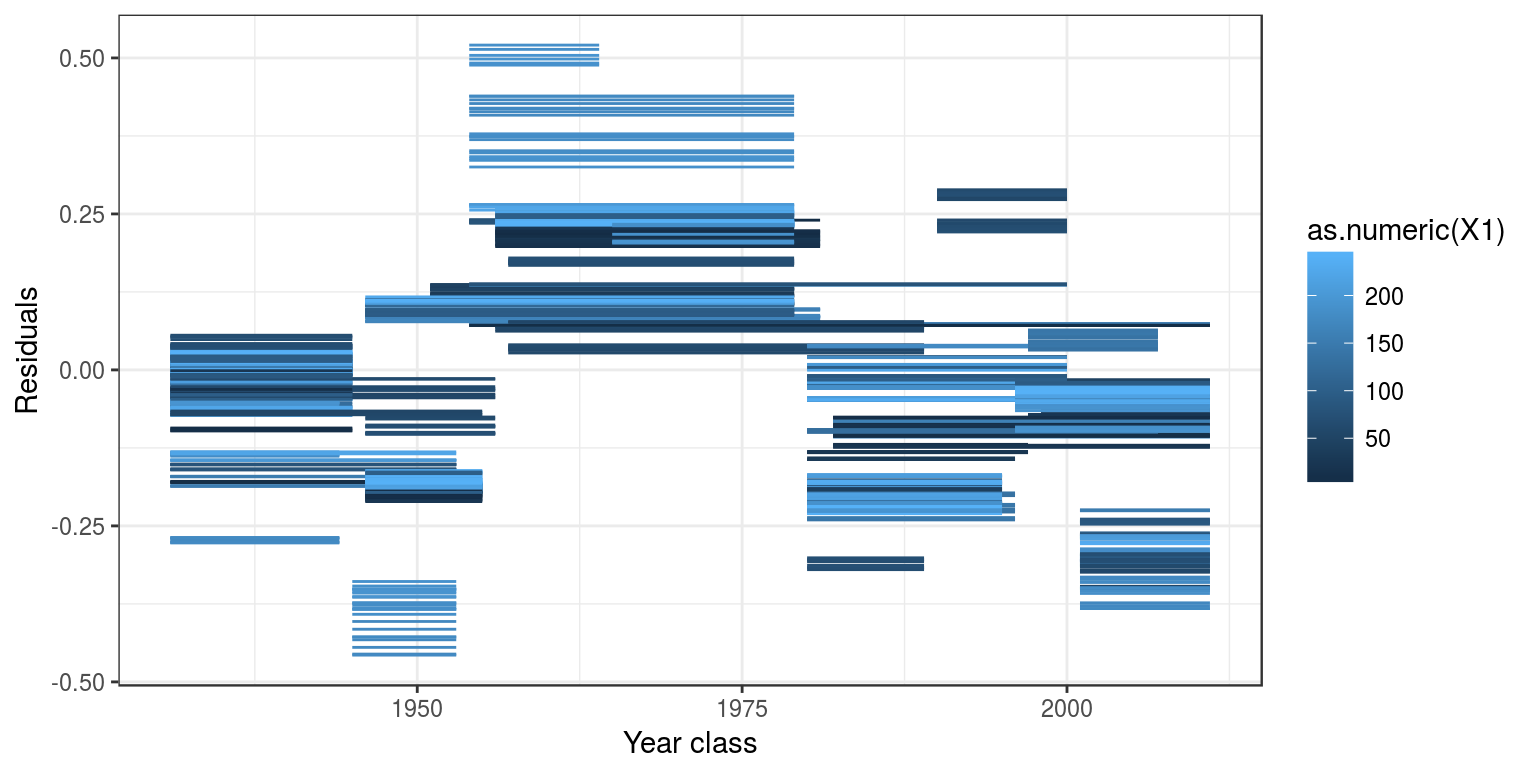
\includegraphics[width=6in]{om-regime.png}
\label{fig:regime}
\caption{Recruitment regimes}
\end{figure*}

\begin{figure*}[htbp]
\centering
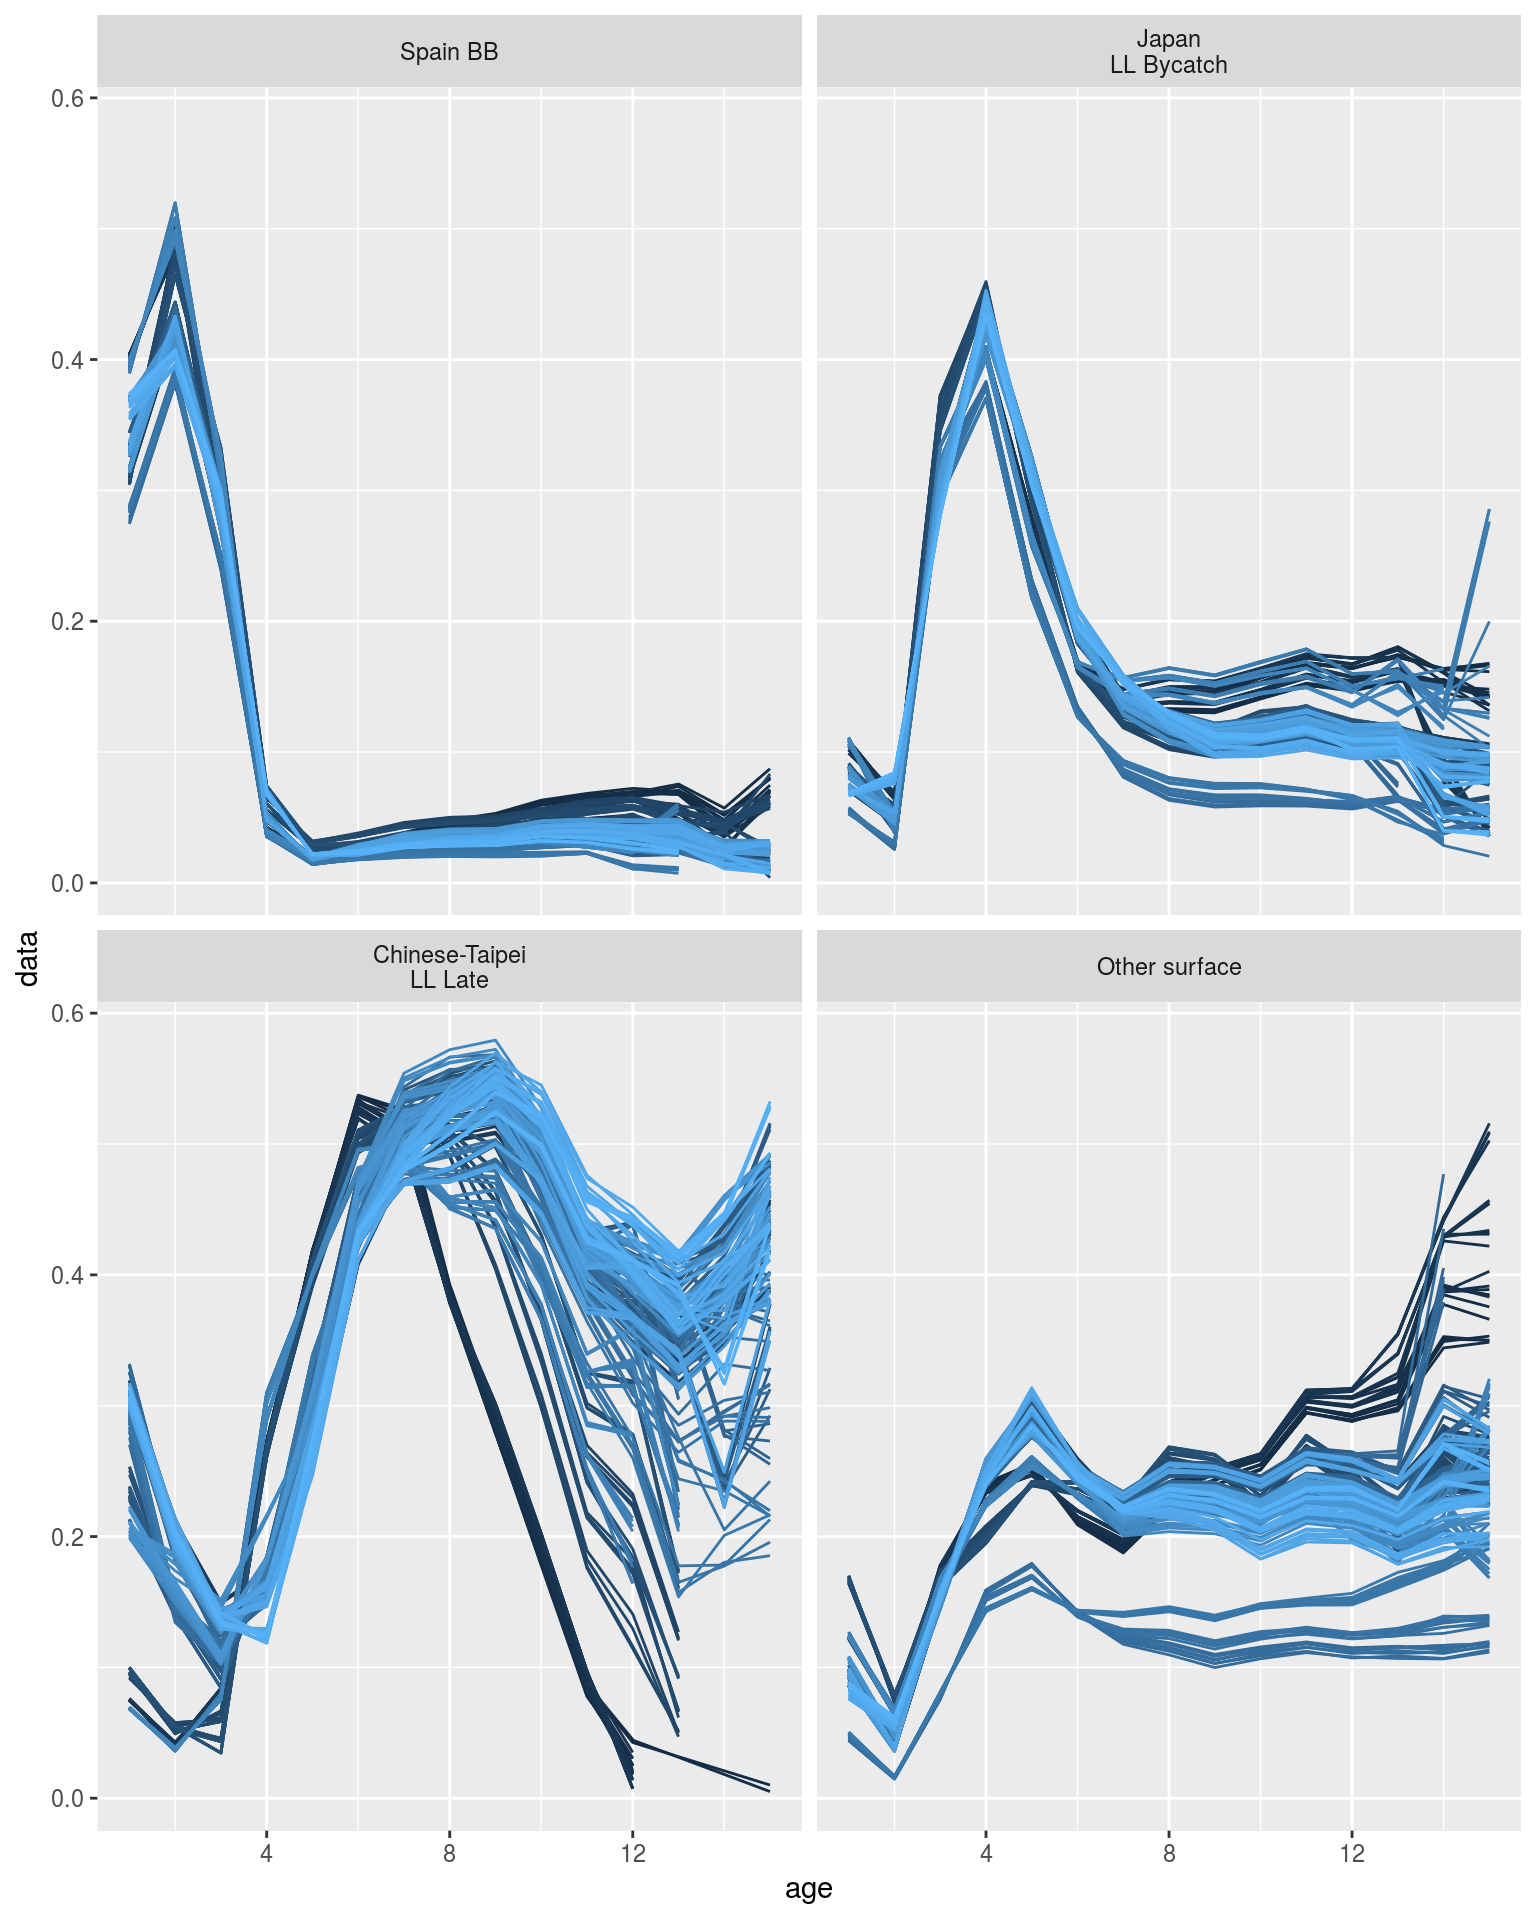
\includegraphics[width=6in]{oem-sel.png}
\label{fig:oem-sel}
\caption{The selection patterns for the four fleets used to condition the Operating Model.}
\end{figure*}

\begin{figure*}[htbp]
\centering
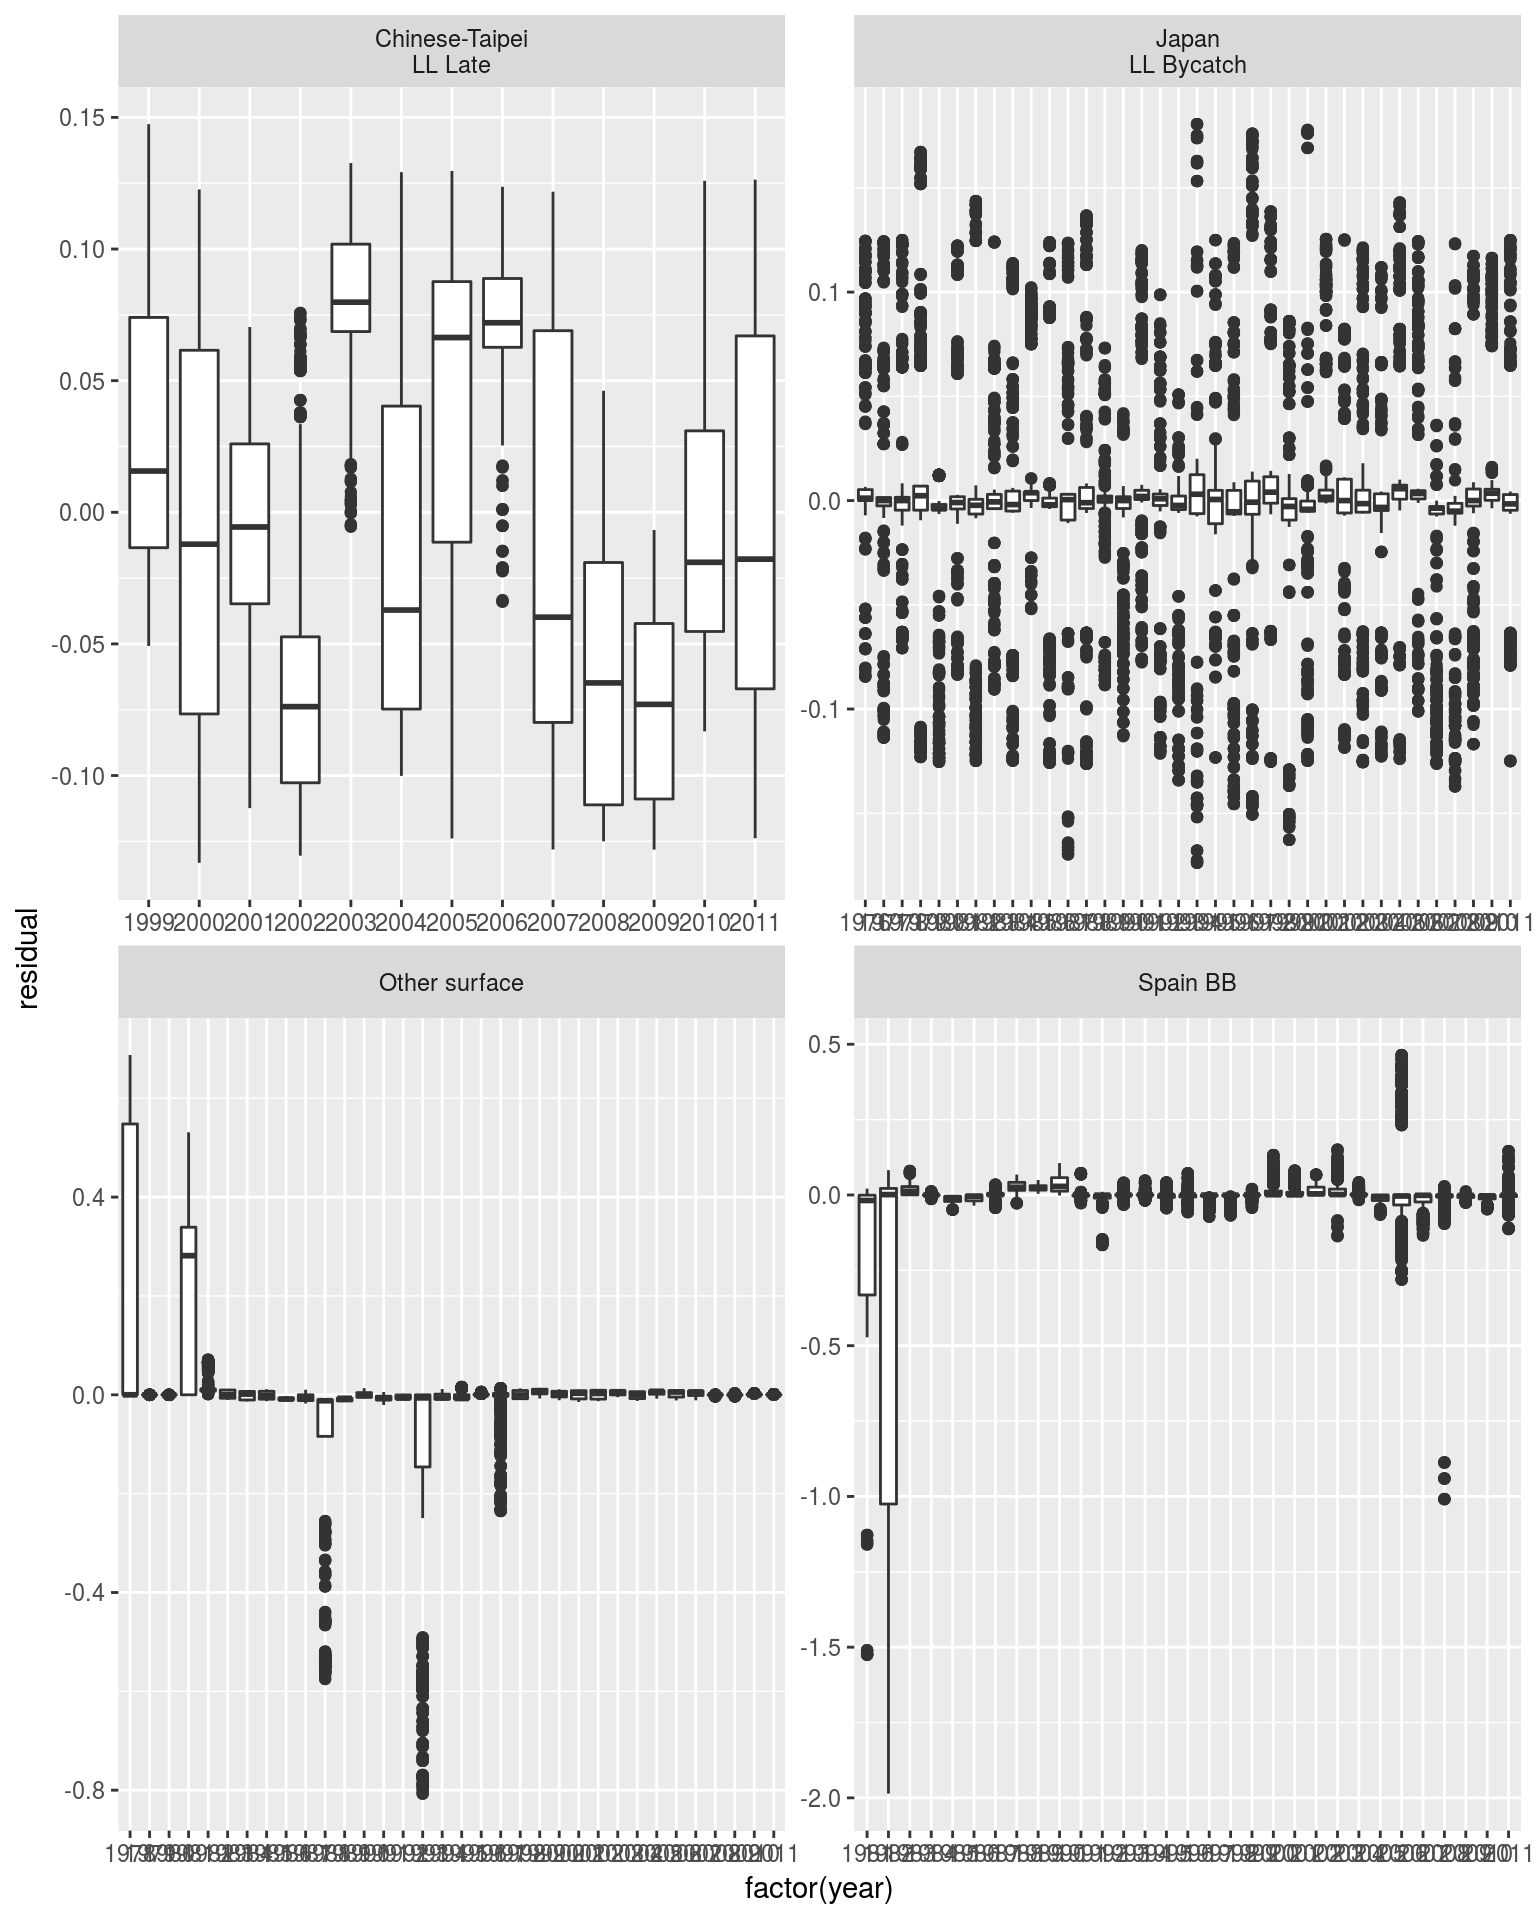
\includegraphics[width=6in]{oem-dev.png}
\label{fig:oem-devs}
\caption{The residuals for the four fleets used to condition the Operating Model.}
\end{figure*}

\begin{figure*}[htbp]
\centering
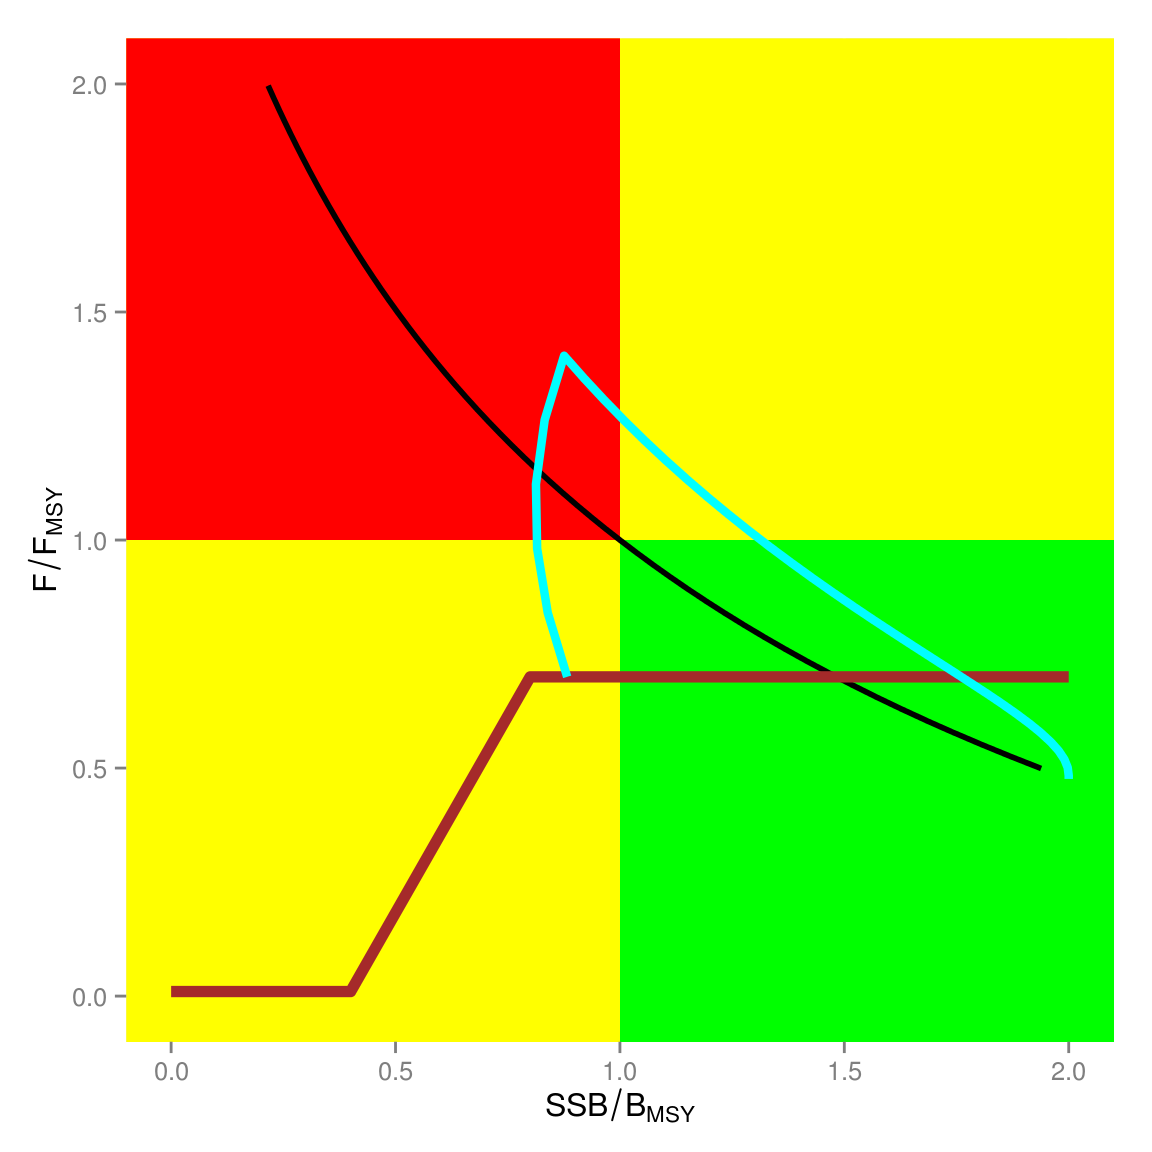
\includegraphics[width=6in]{hcr.png}
\label{fig:hcr}
\caption{Harvest Control Rule (brown) plotted on a phase plot of harvest rate relative to $F_{MSY}$ and stock biomass relative to $B_{MSY}$; the light line is the simulated stock and the black line is the replacement line.}
\end{figure*}

\newpage\clearpage
\section{Appendix}

\newpage\clearpage
\section*{Equations}

\subsection*{Operating Model}

Growth was modelled by the \cite{vonbert1957quantitative} growth equation i.e.
 
\begin{equation} L_t = L_{\infty}(1 - e^{-kt-t_0}) \end{equation} 
 
where $L_{\infty}$ is the asymptotic length attainable, $k$ the rate at which the rate of growth in length declines as length approaches
$L_{\infty}$, and $t_{0}$ is the time at which an individual is of zero length. 
 
Mass-at-age is then derived from length using a scaling exponent ($a$) and the condition factor ($b$)
 
\begin{equation} W_t = a \times W_t^b \end{equation} 
 
Maturity ($Q$) was either based on \cite{santiago2004dinamica}  or derived as in \cite{williams2003implications} 
from the theoretical relationship between $M$, $K$, and age at maturity ($a_{Q}$)  
based on the dimensionless ratio of length at maturity to asymptotic length \citep{beverton1992patterns}. It was then  
modelled by the logistic equation with 2 parameters: age at 50\% ($a_{50}$) and 95\% ($a_{95}$) mature.

\begin{equation}
f(x) = \left\{ \begin{array}{ll}
			0                                 &\mbox{ if $(a_{50}-x)/a_{95} >  5$} \\
			a_{\infty}                        &\mbox{ if $(a_{50}-x)/a_{95} < -5$} \\
			\frac{m_{\infty}}{1.0+19.0^{(a50-x)/{a95})}} &\mbox{ otherwise}
		\end{array}
       \right.
\end{equation}

Natural mortality ($M$) at-age was derived from \cite{lorenzen2002density} and \cite{chen1989age}, i.e.

for Lorenzen
 
\begin{equation}
   M_t=3.00*W_t-0.288
\end{equation}
   
   and Chen-Watanabe
 
\begin{equation}
M_t = \left\{ \begin{array}{ll}
			 \frac{k}{1-e^{-k(t-t_0}}     			&\mbox{ for $t<t_m$} \\
			\frac{k}{a_0}+a_1(t-t_m)+a_2(t-t_m)^2           &\mbox{ for $t<t_m$} \\
		\end{array}
       \right.
\end{equation}

where

\begin{subequations}
$a_0=1-e^{-k(t-t_0)}$  \\

$a_1=ke^{-k(t-t_0)}$ \\  

$a_2=-0.5k^{2e^{(-k(t-t_0))}}$ \\  

$t_m=\frac{1}{k}log(1-e^{-kt_0}) +t_0$ \\
\end{subequations} 
 
Selectivity was modelled using a double normal \citep[see][]{hilborn2000documentation} with three parameters that describe the age at maximum selection ($a1$), the rate at which the left hand limb increases ($sl$) and the right hand limb decreases ($sr$) which allows flat topped or domed shaped selection patterns to be chosen.

\begin{equation}
f(x) = \left\{ \begin{array}{rl}
 2^{-[(x-a_1)/s_L]^2} &\mbox{ if $x<a_1$} \\
 2^{-[(x-a_1)/s_R]^2} &\mbox{ otherwise}
       \end{array} \right.
\end{equation}

Stock recruitment relationships were either \citep{cushing1973dependence}
\begin{equation} R=aS^b \end{equation}

or Beverton and Holt \citep{beverton_dynamics_1993}

\begin{equation} R=\frac{S}{a+bS} \end{equation}

\subsection*{Observation Error Model}


\subsection*{Management Procedure}

The biomass of a stock next year ($B_{t+1}$) is equal to the biomass this year $B_{t}$, less the catch ($C_t$) plus the surplus production ($P_t$) i.e. 

\begin{equation}  B_{t+1}=B_{t}-C_{t}+P_{t}\end{equation}  

$P$ is given by the Pella-Tomlinson surplus production function \citep{pella1969generalized}

\begin{equation}\frac{r}{p}\cdot~B(1-(\frac{B}{K})^p)\end{equation}  

\end{document}

